\section{Lexikalanalys}

Eftersom det skulle skapas ett språk för att skanna \texit{fak.c}, valdes att enbart det alfabet
som \texit{fak.c} använder. Detta gjordes genom att titta på \texit{fak.c}.
\\ \texit{pas.l} användes som en mall för att utveckla språket för specifikt \texit{fak.c} 

\begin{figure}[!h]
    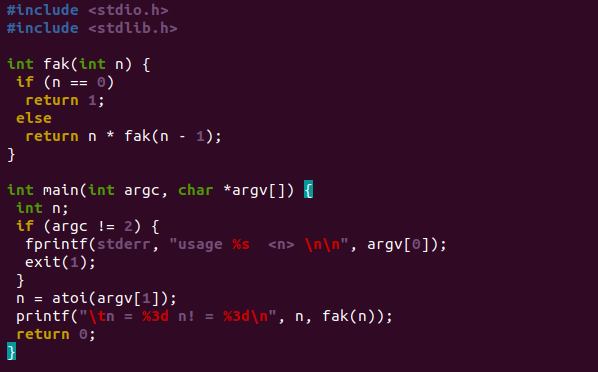
\includegraphics[width=\linewidth,height=3cm]{bilder/fak.c.png}
    \captionof{figure}{fak.c koden}
    \label{fig:fak.c}
\end{figure}

